\section{Introduction}
The generation of a pair of entangled photons from the biexcition-exciton cascade is complicated by the presence of fine structure splitting (FSS)\cite{Winik2017} that leads to the degradation of the degree of entanglement. Many methods were implemented to overcome the problem with varying degrees of success, but the problem continues to persist.  \\ \\
This research proposal aims to take a different approach to the problem by implementing a scheme for the restoration of the degree of entanglement of the photon pairs by fast polarization manipulation \cite{Fognini18,Varo2022}.\\
This scheme can be potentially used as a method for fast photon rerouting in integrated photonics.   

	
  	

\subsection{The QD exciton fine structure}
Figure \ref{fig:energy_structure}  presents the four lowest energy configurations of electron-heavy hole pairs (excitons) and describes the energy difference between the parallel and anti-parallel spin configurations. The energy splitting between the DE and the BE is $\triangle_0 \approx 300 \mu eV$ due to the isotropic long and short-range electron-hole exchange interaction (EHEI). Additional splitting is caused by the anisotropic (mainly long-range) EHEI, which removes the degeneracy between the two BE eigenstates by $\triangle_2 \approxeq 30 \mu eV $.The BE eigenstates are the symmetric and the antisymmetric configurations of the electron and hole with anti-parallel spins $ \ket{S}_{BE} = (\ket{\uparrow\Downarrow}+(\downarrow\Uparrow))/\sqrt{2}$ and  $ \ket{A}_{BE} = (\ket{\uparrow\Downarrow}-(\downarrow\Uparrow))/\sqrt{2}$ respectively. Here, a single arrow represents an electron and a double arrow represents a heavy hole in their respective ground levels. The DE eigenstates, similar to that of the BE, are the symmetric and the anti-symmetric configurations of the electron–hole pair with parallel spins $ \ket{S}_{DE} = (\ket{\uparrow\Uparrow}+(\downarrow\Downarrow))/\sqrt{2}$ and $ \ket{A}_{DE} = (\ket{\uparrow\Uparrow}-(\downarrow\Downarrow))/\sqrt{2}$.
\begin{figure}[H]
	\centering
	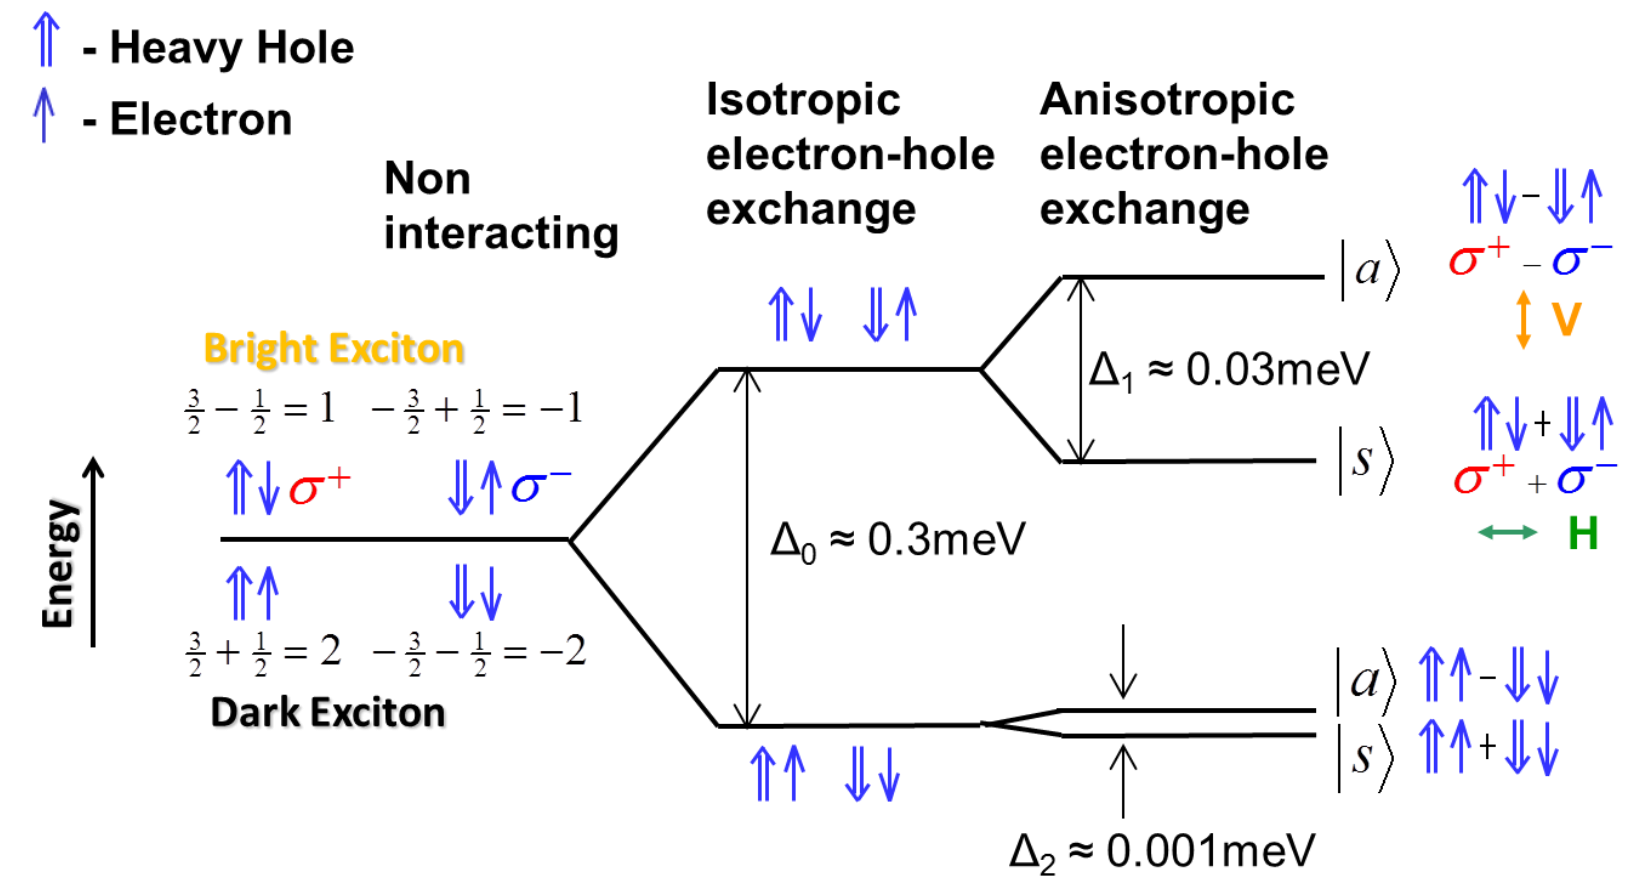
\includegraphics[scale=0.32]{figures/energy_structure.png}
	\caption{Schematic description of the bright and dark exciton energy levels and spin eigenstates. The polarization of light that interacts with the BE eigenstates is marked underneath the corresponding BE eigenstate.}
	\label{fig:energy_structure}
\end{figure}
Both the BE and DE thus have two non-degenerate spin eigenstates and both can, under some approximation, be considered as an isolated physical two level system. An exciton in an eigenstate will eventually decay. The BE which isoptically allowed, decays radiatively within $\approx$1 ns.The DE, which isoptically forbidden, lives much longer. A lowest limit for the DE lifetime was experimentally deduced in Ref. \cite{McFarlane2009} and by Schwartz \cite{Schwartz_2015}.Theoretical estimations of this lifetime, assuming heavy-hole - light-hole mixing, which opens a small channel for radiative recombination are recently published by Korkusinski \cite{Korkusinski2013} and Zielinsky \cite{Zielinski2013}. The two eigenstates of the BE are equally optically allowed and therefore both have roughly the same lifetime. In contrast, the DE lifetime is determined by the mixing of the heavy-hole with the light hole. This mixing is constructive for one DE eigenstate and destructive for the other. Thus one DE eigenstate is darker than the other.
27]
Figure ‎1.1: Schematic description of the bright and dark exciton energy levels and spin eigenstates. The polarization of light that interacts with the BE eigenstates is marked underneath the corresponding BE eigenstate.4
In a physical two-level system, according to quantum mechanics, any superposition of the two eigenstates is an allowed state of the system. Such a state, decays like the eigenstates. In addition, however, due to the energy difference between the two eigenstates, the relative phase between them varies in time. This temporal evolution can be described as a precession (Larmor precession) of the state vector at an angular frequency which is given by the energy difference between the two eigenstates divided by the Planck constant. The precession lasts as long as the physical system lives and maintains its coherence. In other words, the phase between the two eigenstates is not destroyed by interactions of the system with its environment. The BE precession time of ~100 psecs was measured by Benny et al [20]. The DE precession time of ~3 nsec was measured by Poem et al. [22]. The spin coherence time of the BE is much longer than its radiative lifetime,and therefore, cannot be directly measured. The first lowest bound measurement for the DE coherence time is presented in the preliminary results section of this research proposal.
Quantum information processing is based on replacing the classical information bit (either 0 or 1) by a physical two level system or a quantum bit(Qubit). The BE and the DE are thus potential candidates for Qubits. [20, 22,28]
\subsection{Pulsed On-Demand Sources of Photonic Cluster State Strings }
	The projection of the spin of the electron on the z-axis (growth axis) of the QD can be either 1/2 or -1/2 while for the heavy hole, the spin 
 projection is either 3/2 or -3/2 such that the two spin states of the bright exciton are $\ket{\frac{1}{2},-\frac{2}{3}}$ and $\ket{-\frac{1}
 {2},\frac{2}{3}}$  with a total spin in the z direction  of $\pm1$. While in the case of electron-hole pair with parallel spin, the spin states are $\ket{\frac{1}{2},\frac{2}{3}}$ and $\ket{-\frac{1}{2},-\frac{2}{3}}$ with a total spin of $\pm2$.\\
	In figure \ref{fig:energy_levels} we describe two of the simple configurations that we can have in a QD. We start with an empty dot which we denote by $\ket{0}$.
	\begin{figure}[H]
		\centering
		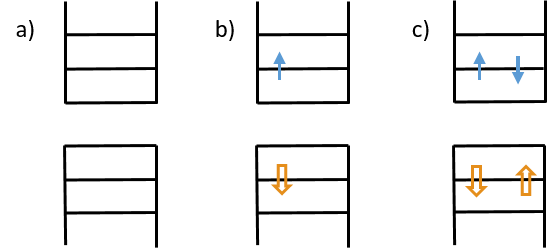
\includegraphics[scale=1]{figures/energy-levels.png}
		\caption{Schematic of the energy levels in the quantum dot for empty quantum dot (a),exciton (b) and a biexciton (c)}
		\label{fig:energy_levels}
	\end{figure}
	while having two electron-hole pairs falling in the dot a biexciton is formed and we denote it by $\ket{{XX}_0}$. The total energy of the biexciton differs from twice the energy of the exciton due to the interaction between all the particles.\\
	
	In an ideal QD, the radiative decay path of the biexciton back to the ground state goes via one path, but due to the anisotropy of the QD, the energy of exciton is split in what is defined as the fine structure splitting (FSS) as seen in figure \ref{fig:figureDecay_paths}b. Here we refer to the up (down) spin of the electron as $\ket{\uparrow}$ ($\ket{\downarrow}$ and the up (down) spin of the hole as $\ket{\Uparrow}$ ($\ket{\Downarrow}$ such as the two eigenstates of the exciton are  $\ket{\uparrow\Downarrow}$ and $\ket{\downarrow\Uparrow}$, and the decay from these states result in the emission of photons with co-linear polarization. Here we refer to them as horizontal $\ket{H}$ and vertical $\ket{V}$. We can represent these two rectilinear bases using the Bloch sphere where the poles in the sphere are $\ket{H}$ and $\ket{V}$ bases.\\
	
	In addition to the rectilinear polarization states, We can define the diagonal linear and
	the circular polarization bases: 
	\begin{equation}
		\begin{split}
			\ket{L}=(\ket{H}+i\ket{V})/\sqrt{2} \\
			\ket{R}=(\ket{H}-i\ket{V})/\sqrt{2}
		\end{split}
	\end{equation}
	where $\ket{R}$ and $\ket{L}$ are the left and right circular bases respectively, and:
	\begin{equation}
		\begin{split}
			\ket{D}=(\ket{H}+\ket{V})/\sqrt{2}\\
			\ket{\bar{D}}=(\ket{H}+\ket{V})/\sqrt{2}
		\end{split}
	\end{equation}
	$\ket{D}$ and $\ket{\bar{D}}$ are the diagonal and anti-diagonal bases respectively
	
	\begin{figure}[H]
		a)
		\raggedleft
		\def\psiLat{0}
		\def\psiLon{-50}
		\begin{blochsphere}[radius=2.5 cm,tilt=20,rotation=-20,opacity=0]
			\labelLatLon{psi}{\psiLat}{-\psiLon};
			\draw[-latex] (0,0) -- (psi) node[above]{$\large\ket{\psi}$};
			\drawRotationLeft[scale=0.9,style={red}]{0}{0}{0}{15}
			
			\drawGreatCircle[style={dashed}]{0}{0}{0}
			\drawBallGrid[style={opacity=0.5}]{30}{30}
			\draw [fill] (0,0) circle (1.5pt);
			\drawGreatCircle[style={dashed}]{0}{0}{0}
			\labelLatLon{up}{90}{0};
			\labelLatLon{down}{-90}{90};
			\node[above] at (up) {{ $\ket{H}$ }};
			\node[below] at (down) {{ $\ket{V}$}};
			\node at (2.8,0) {{$\ket{R}$}};
			\node at (-2.8,0) {{$\ket{L}$}};
			\node at (0,1) {{$\ket{D}$}};
			\node at (0,-1) {{$\ket{\bar{D}}$}};
		\end{blochsphere}
		b)
		\raggedright
		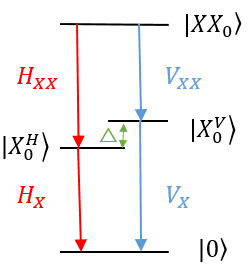
\includegraphics[scale=0.8]{figures/Decay_paths.png}
		\caption{a) A Bloch sphere representation of the spin state. A point on the sphere represents an arbitrarily polarized spin state. b) Decay paths of the biexciton back the ground state where the red arrows represent the emission of a H polarized photon and blue arrows represent the emission of V polarized photon.}
		\label{fig:Decay_paths}
	\end{figure}
	When the biexciton spontaneously radiatively decays it  emits a photon leaving 
	in the QD an exciton in coherent superposition of its two eigenstates. The optical
	selection rules for the biexciton radiative recombination and the lack of information by “which path” the recombination proceeds result in entanglement between the exciton state and the polarization state of the emitted photon. Their mutual wave function is given by:
	\begin{equation}
		\ket{\psi_{X^0}} = \frac{1}{\sqrt{2}}(\ket{H_1H^1_H} +\ket{V_1V^1_V})
	\end{equation}
	here $\ket{H_1}$ and $\ket{V1}$ are the two rectilinear polarization states of the first (biexciton) photon. since the two exciton eigenstates are not degenerate, the relative phase between these eigenstates precesses in time with a period of $T_P = h/\triangle$, where where $h$ is the Planck constant and $\triangle$ is the exciton FSS \cite{rwinik2017}.
	This precession is schematically described on the exciton Bloch sphere in figure. $\ref{fig:Decay_paths}a$.
	The precession “stops” when the exciton recombines and the radiative cascade is completed with the emission of a second photon. The two photons are thus entangled. Their mutual wave function depends on the recombination time and is given by:
	\begin{equation}
		\ket{\psi_{X^0}} = \frac{1}{\sqrt{2}}(\ket{H_1H_1} +e^{-i2\pi t/T_P}\ket{V_1V_2})
	\end{equation}
 
	where $\ket{H_2}$ and $\ket{V_2}$ are the second (exciton) photon polarization states and $t = t_{X_0} - t_{{XX}_0}$ is the time between the emission of the biexciton photon $t_{{XX}_0}$ and that of the exciton $t_{X_0}$.